\documentclass[12pt,a4paper]{article}

\usepackage{fontspec}
\usepackage{geometry}
\geometry{left=25mm, right=15mm, top=20mm, bottom=20mm}
\usepackage{graphicx}
\usepackage{booktabs}
\usepackage{longtable}
\usepackage{array}
\usepackage{hyperref}
\usepackage{caption}
\usepackage{float}
\usepackage{enumitem}
\usepackage{multirow}
\usepackage{xcolor}
\usepackage{colortbl}
\usepackage{amsmath}

\setmainfont{DejaVu Serif}
\setsansfont{DejaVu Sans}
\setmonofont{DejaVu Sans Mono}

\hypersetup{colorlinks=true, linkcolor=blue, urlcolor=blue}

\graphicspath{{../results/}}

\title{
  \vspace{-1cm}
  \textbf{Profiling Vision-Language Models}\\[0.3cm]
  \large Performance, energy, and output quality
}
\author{Vladislav Smirnov}
\date{March 2026}

\begin{document}
\maketitle

\vspace{-0.5cm}
\noindent\textbf{Repository:} \url{https://github.com/smirnovlad/vlm-profiler}

\tableofcontents
\newpage

% ============================================================
\section{Introduction}

This project measures how different Vision-Language Models (VLMs) behave under varying conditions: image resolution, prompt length, batch size, hardware, and optimization settings.  We record latency, FLOPs, GPU energy draw, and Word Error Rate (WER) on three datasets, then compare the models head to head.

\subsection{Hardware}
\begin{itemize}[nosep]
  \item 2$\times$ NVIDIA RTX 5880 Ada, 48\,GB VRAM each
  \item Python 3.13, conda environment
  \item PyTorch + HuggingFace Transformers
\end{itemize}

% ============================================================
\section{Experiment plan}
\label{sec:plan}

\subsection{Models}

We test 7 models that cover the main VLM families available on HuggingFace:

\begin{table}[H]
\centering
\caption{Models used in this study.}
\begin{tabular}{@{}clcc@{}}
\toprule
\# & Model & Parameters & Backbone \\
\midrule
1 & \texttt{blip2-opt-2.7b} & 3\,745M & BLIP-2 + OPT \\
2 & \texttt{blip2-flan-t5-xl} & 3\,942M & BLIP-2 + Flan-T5 \\
3 & \texttt{instructblip-flan-t5-xl} & 4\,023M & InstructBLIP + Flan-T5 \\
4 & \texttt{instructblip-vicuna-7b} & 7\,914M & InstructBLIP + Vicuna \\
5 & \texttt{llava-1.5-7b-hf} & 7\,063M & LLaVA 1.5 (7B) \\
6 & \texttt{llava-1.5-13b-hf} & 13\,351M & LLaVA 1.5 (13B) \\
7 & \texttt{fuyu-8b} & 9\,408M & Fuyu (8B) \\
\bottomrule
\end{tabular}
\end{table}

We originally planned to include \texttt{HuggingFaceM4/idefics2-8b} but dropped it: every generation call crashed with a pixel-values shape mismatch (``not enough values to unpack (expected 5, got 4)'') against \texttt{transformers} 5.x. Fixing the integration is tracked separately and is not in the scope of this report.

\subsection{Datasets}

Three datasets, 300 samples each:

\begin{table}[H]
\centering
\caption{Evaluation datasets.}
\begin{tabular}{@{}lll@{}}
\toprule
Dataset & Task & Split \\
\midrule
ScienceQA & Visual question answering & validation \\
TextVQA & VQA with text in images & validation \\
COCO Captions & Image captioning & validation \\
\bottomrule
\end{tabular}
\end{table}

\subsection{What we vary}

We use a vary-one-axis design: one parameter changes at a time while the rest stay at baseline values (resolution 224, prompt length 10, batch 1, no optimization, GPU).

\begin{table}[H]
\centering
\caption{Scaling axes.}
\begin{tabular}{@{}llc@{}}
\toprule
Axis & Values & Baseline \\
\midrule
Image resolution & 224, 336, 448, 512 & 224 \\
Prompt length (tokens) & 10, 50, 100, 200 & 10 \\
Batch size & 1, 2, 4, 8 & 1 \\
Optimizations & none, FP16, torch.compile & none \\
Device & CUDA, CPU & CUDA \\
\bottomrule
\end{tabular}
\end{table}

\subsection{Metrics}

\begin{enumerate}[nosep]
  \item \textbf{Latency (ms)} --- wall-clock time per inference (3 warmup + 10 timed runs).
  \item \textbf{FLOPs} --- measured with calflops where possible; otherwise estimated as $2 \times \text{params}$.
  \item \textbf{Energy (J per inference)} --- GPU power sampled via \texttt{nvidia-smi} at 100\,ms intervals, integrated over inference time.
  \item \textbf{WER} --- Word Error Rate between the model output and the reference answer.
\end{enumerate}

\subsection{Total number of runs}

Each (model, dataset) pair produces roughly 15 experiments:
\begin{itemize}[nosep]
  \item 1 baseline (all metrics)
  \item 3 extra resolutions
  \item 3 extra prompt lengths
  \item 3 extra batch sizes
  \item 2 optimization variants (FP16, torch.compile)
  \item 1 CPU run
\end{itemize}
That gives about 330 successful experiments across 7 models and 3 datasets.

% ============================================================
\section{Weekly schedule}
\label{sec:schedule}

\begin{table}[H]
\centering
\caption{Work schedule.}
\begin{tabular}{@{}cp{10cm}@{}}
\toprule
Week & What got done \\
\midrule
1 &
  Set up conda + CUDA environment and dependencies.
  Wrote data loading (\texttt{loader.py}, \texttt{preprocessing.py}) and the model registry (\texttt{registry.py}). \\
\midrule
2 &
  Built profiling modules (latency, FLOPs, energy, quality).
  Wrote the experiment runner.
  Ran smoke tests on all 8 models. \\
\midrule
3 &
  Ran the full experiment matrix on 2 GPUs.
  Debugged FP16 dtype errors, OOM crashes, and torch.compile failures on T5 models.
  Re-ran failed experiments.
  Generated report and charts. \\
\midrule
4 &
  Analyzed results and wrote up findings.
  Compared with numbers from original papers.
  Compiled the final PDF report. \\
\bottomrule
\end{tabular}
\end{table}

% ============================================================
\section{Experiment 1: baseline comparison}
\label{sec:experiment1}

\subsection{Setup}

All models run at resolution 224, prompt length 10 tokens, batch size 1, FP32, on GPU.  We measure all four metrics on each of the three datasets.

\subsection{Baseline results}

\begin{table}[H]
\centering
\caption{Baseline comparison (batch=1, res=224, GPU).}
\begin{tabular}{@{}lrrrr@{}}
\toprule
Model & Latency, ms & WER & Energy, J & Params \\
\midrule
blip2-opt-2.7b          &   115.24 & 1.39 &  29.34 & 3\,745M \\
blip2-flan-t5-xl        &   135.75 & 1.21 &  31.21 & 3\,942M \\
instructblip-flan-t5-xl &   329.69 & 1.33 &  69.56 & 4\,023M \\
fuyu-8b                 & 1\,562.25 & 6.21 & 403.91 & 9\,408M \\
llava-1.5-7b-hf         & 1\,654.08 & 6.38 & 450.39 & 7\,063M \\
llava-1.5-13b-hf        & 1\,704.07 & 6.46 & 470.38 & 13\,351M \\
instructblip-vicuna-7b  & 1\,792.87 & 6.17 & 486.71 & 7\,914M \\
\bottomrule
\end{tabular}
\end{table}

What stands out:
\begin{itemize}[nosep]
  \item The BLIP-2 and InstructBLIP-T5 models finish in 115--330\,ms.  The 7B+ models (LLaVA, Vicuna, Fuyu) take 10--15$\times$ longer, around 1.5--1.8\,s.
  \item \texttt{blip2-flan-t5-xl} has the lowest WER (1.21) and is the second fastest model.
  \item Energy tracks latency almost linearly: the fast group uses about 30\,J per inference, the slow group 400--490\,J.
\end{itemize}

\subsection{WER by dataset}

\begin{table}[H]
\centering
\caption{Per-dataset WER (lower is better).}
\begin{tabular}{@{}lrrr@{}}
\toprule
Model & COCO Caption & ScienceQA & TextVQA \\
\midrule
blip2-flan-t5-xl        & 0.79 &  1.30 & 1.54 \\
blip2-opt-2.7b          & 0.82 &  1.49 & 1.87 \\
instructblip-flan-t5-xl & 1.85 &  1.28 & 0.86 \\
instructblip-vicuna-7b  & 0.96 & 11.18 & 6.36 \\
fuyu-8b                 & 4.65 &  6.42 & 7.57 \\
llava-1.5-7b-hf         & 3.37 &  7.02 & 8.75 \\
llava-1.5-13b-hf        & 3.36 &  7.96 & 8.06 \\
\bottomrule
\end{tabular}
\end{table}

A few things to note:
\begin{itemize}[nosep]
  \item \texttt{instructblip-flan-t5-xl} gets the best WER on TextVQA (0.86) but is worse on captioning.
  \item \texttt{instructblip-vicuna-7b} does well on COCO Caption (0.96) but struggles on ScienceQA (11.18).  It seems to have trouble with science-style questions.
  \item The T5-based models are consistently good across all three datasets.
\end{itemize}

\subsection{Charts}

\begin{figure}[H]
\centering
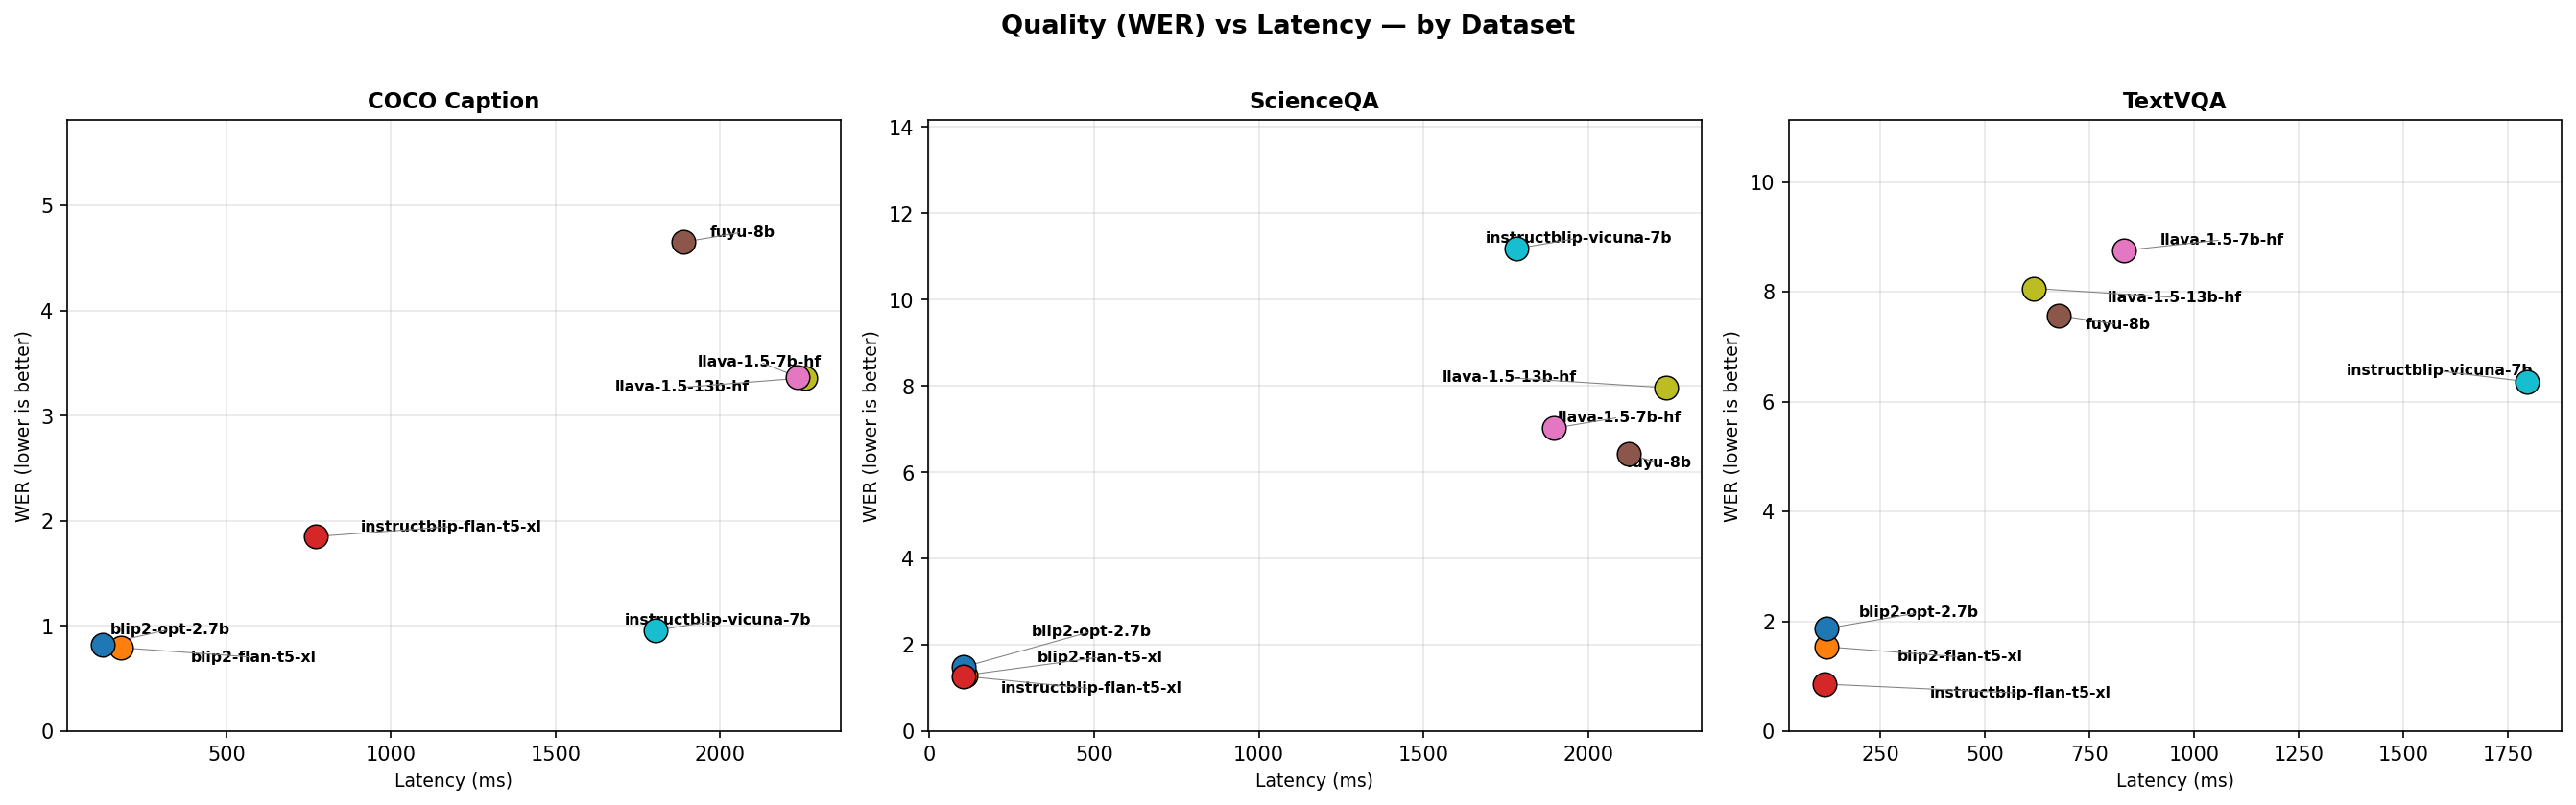
\includegraphics[width=\textwidth]{quality_vs_latency_by_dataset.png}
\caption{WER vs.\ latency, split by dataset.  The dashed line is the Pareto front.}
\end{figure}

On all three datasets the picture is similar: BLIP-2 and InstructBLIP-T5 sit in the bottom-left corner (low WER, low latency), while the 7B+ models cluster in the upper right.  The one exception is \texttt{instructblip-vicuna-7b} on ScienceQA, where it jumps to WER~11 despite having reasonable COCO and TextVQA scores.

\begin{figure}[H]
\centering
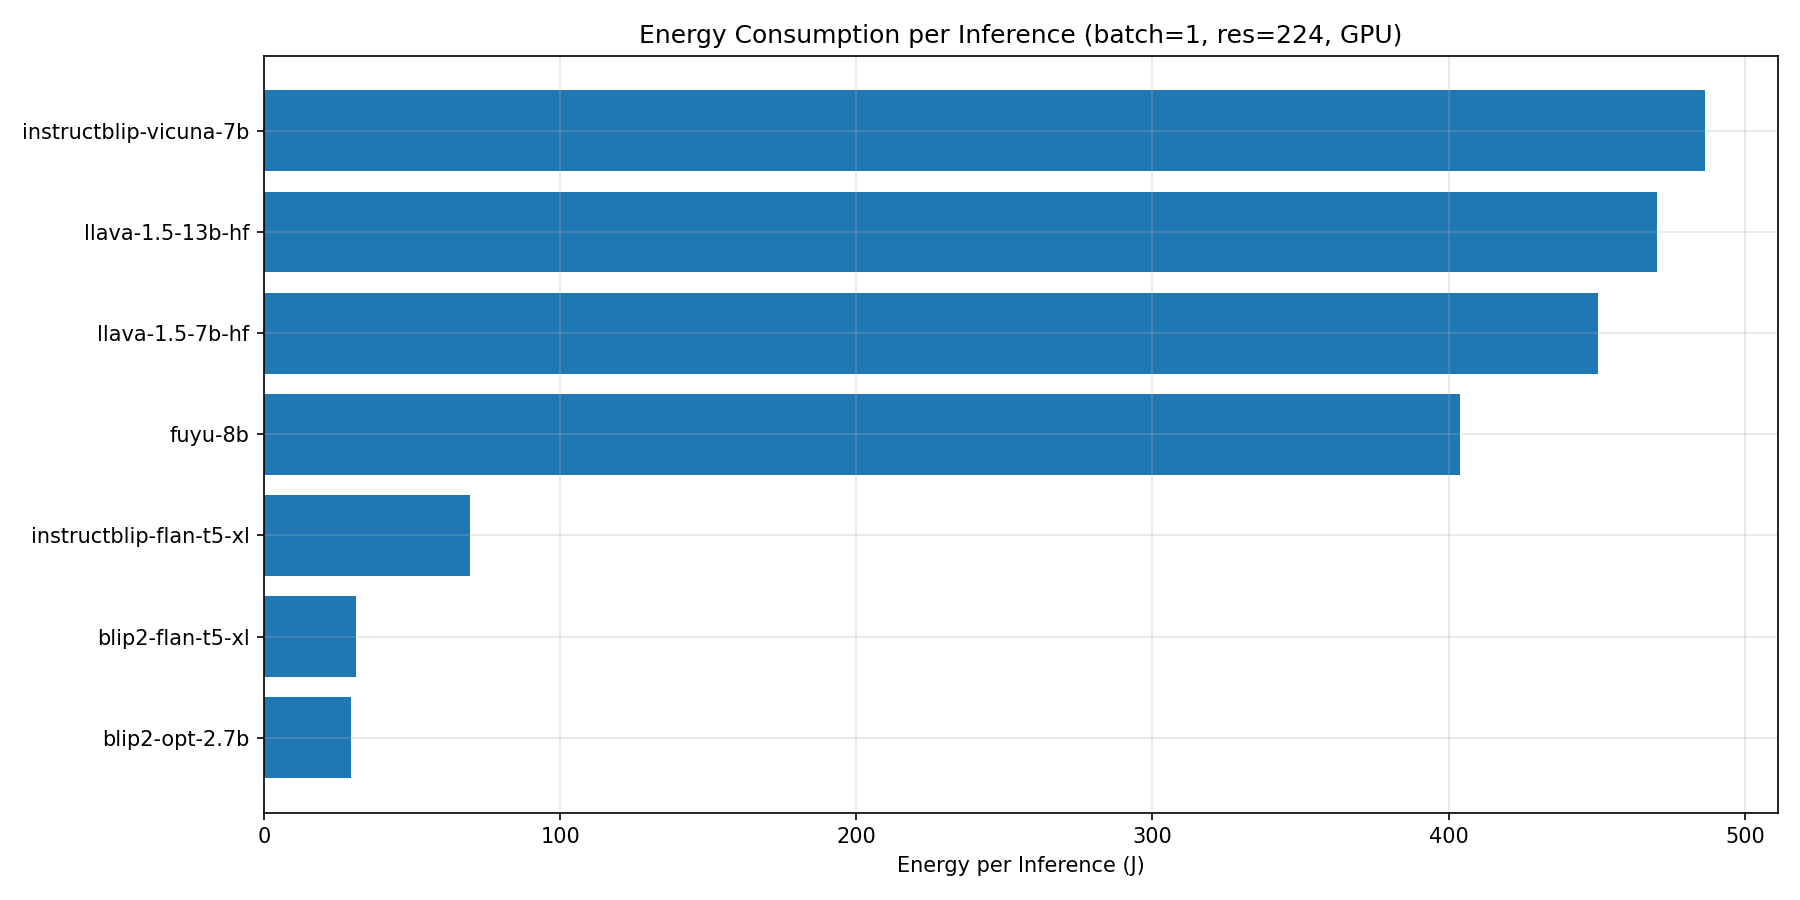
\includegraphics[width=0.85\textwidth]{energy_comparison.png}
\caption{Energy per inference in joules.}
\end{figure}

Energy consumption mirrors latency almost exactly. The three fast models use 29--70\,J per inference, while the 7B+ group sits at 400--490\,J.  There is a clear 6--15$\times$ gap between the two groups.

\begin{figure}[H]
\centering
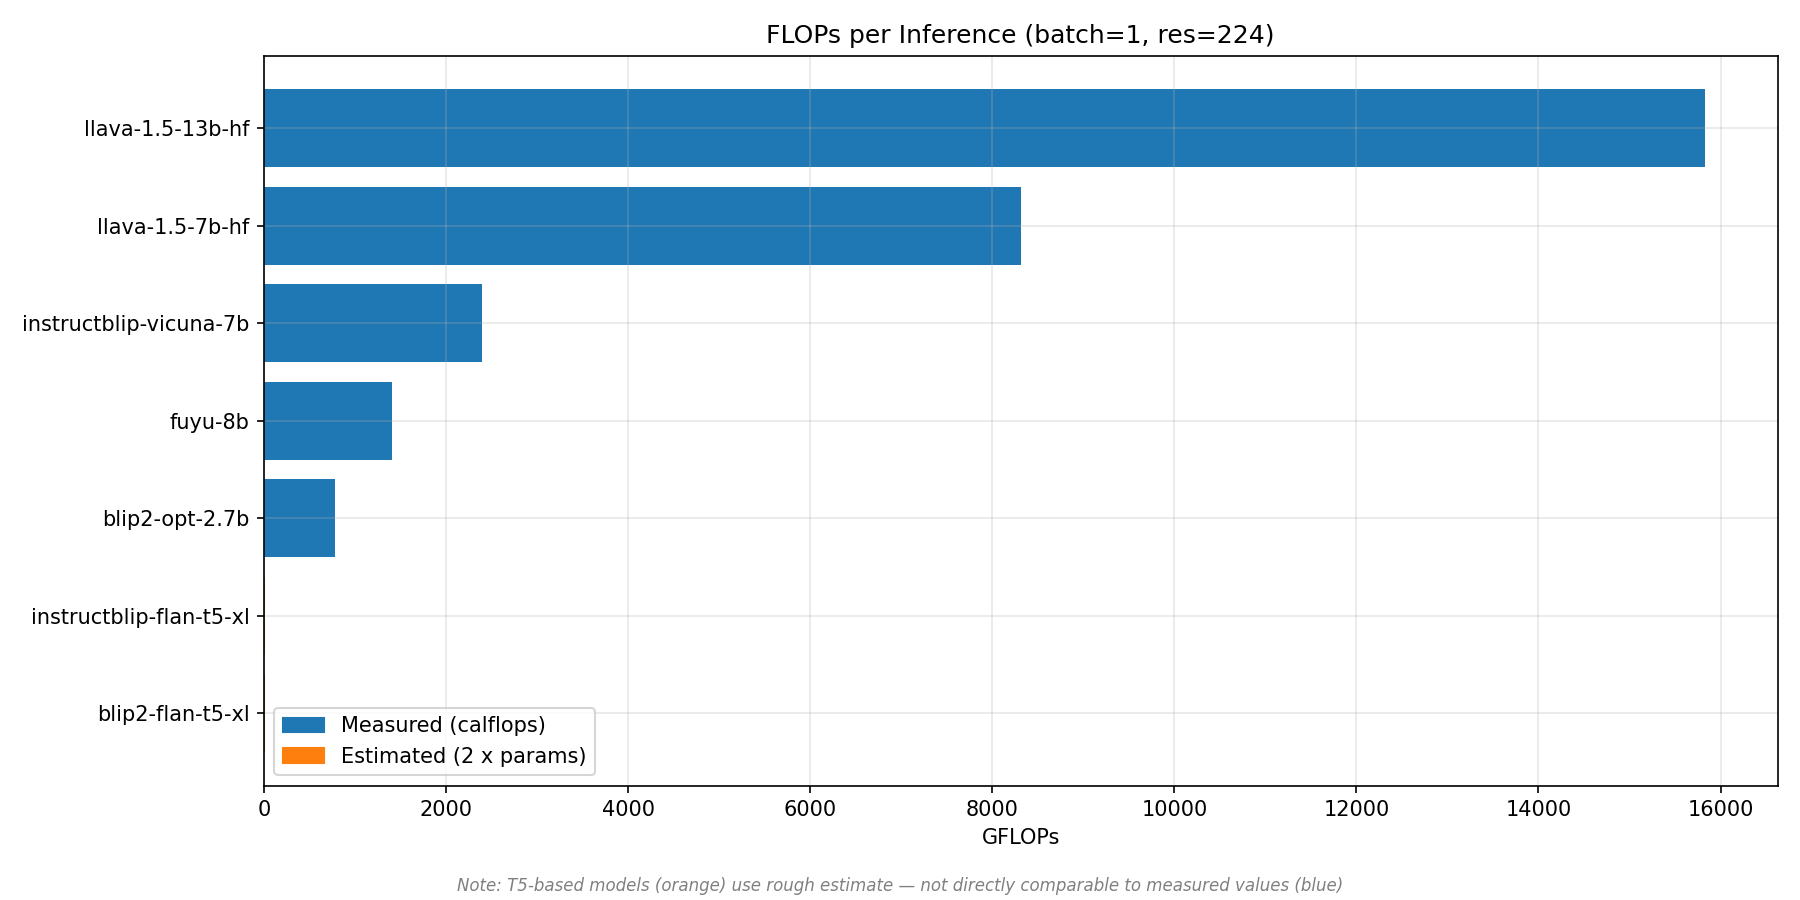
\includegraphics[width=0.85\textwidth]{flops_comparison.png}
\caption{FLOPs per inference.  Blue bars are measured (calflops), orange bars are estimated ($2 \times \text{params}$).}
\end{figure}

The FLOPs chart should be read with caution: blue bars (calflops) and orange bars ($2 \times \text{params}$ estimate) are not directly comparable.  Among the measured models, LLaVA-13B and idefics2-8b have the highest FLOPs, which matches their large decoder sizes. The T5-based models report low estimates because the $2 \times \text{params}$ heuristic is a rough lower bound for encoder-decoder architectures.

\begin{figure}[H]
\centering
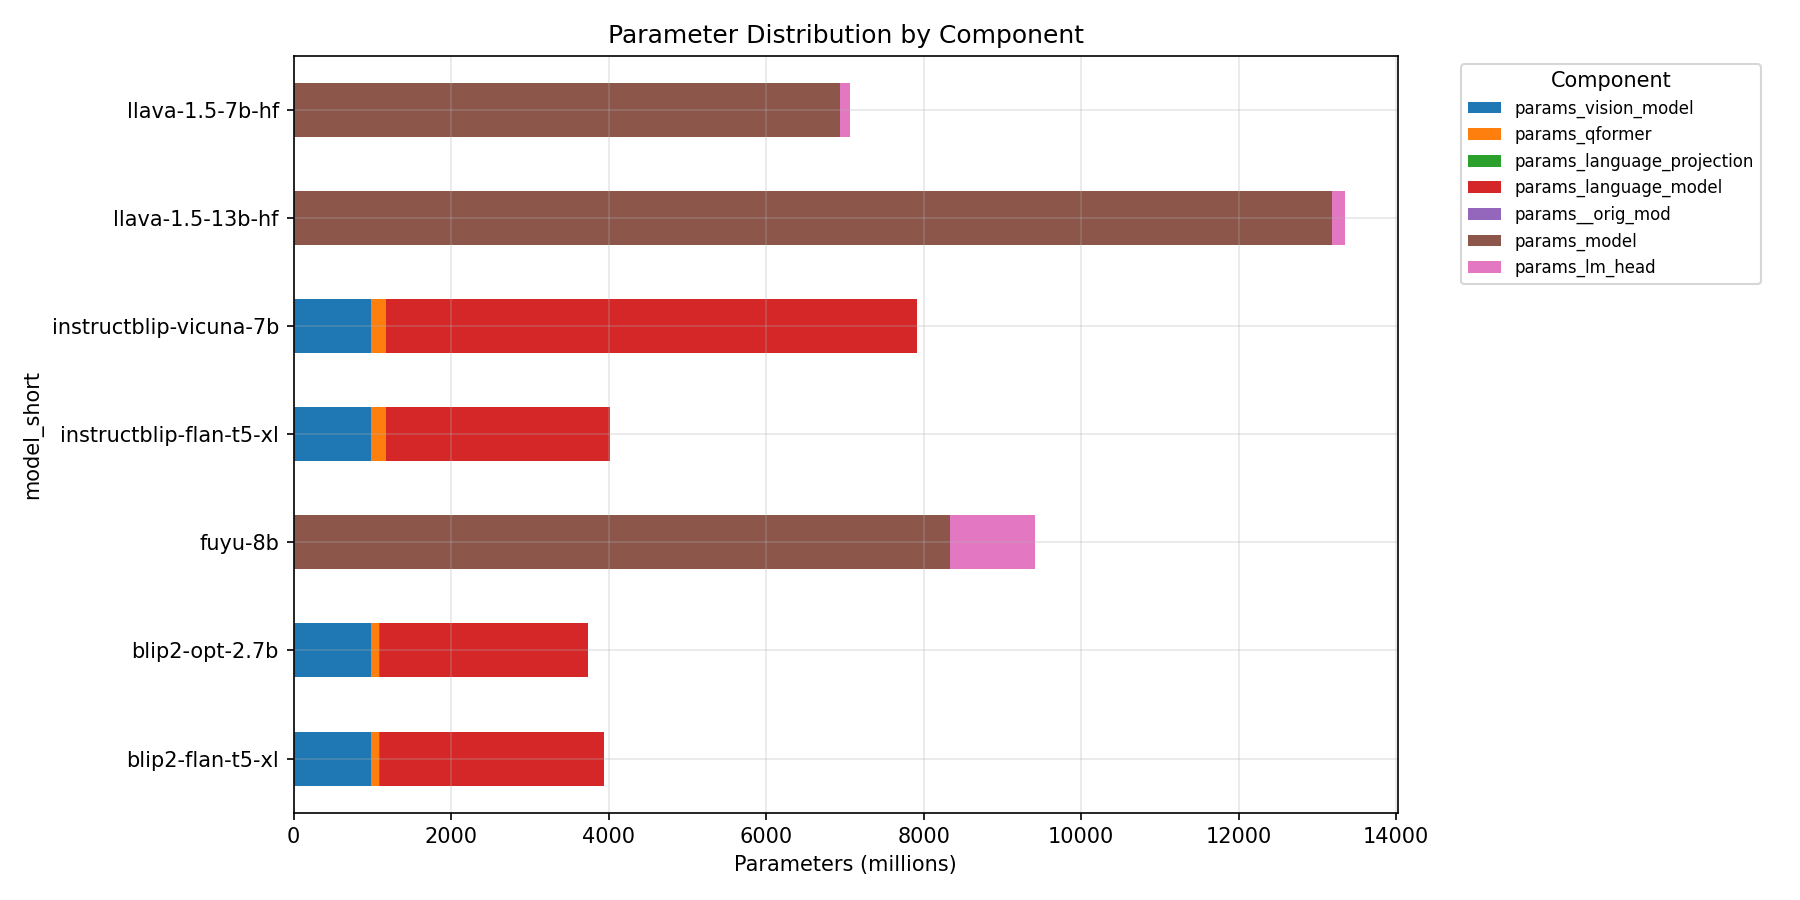
\includegraphics[width=0.85\textwidth]{param_breakdown.png}
\caption{Parameter count broken down by model component.}
\end{figure}

In every model the language decoder accounts for the majority of parameters.  The vision encoder is comparatively small (usually under 400M).  This matches the latency results: the LLM backbone is the bottleneck, not the image encoder.

\begin{figure}[H]
\centering
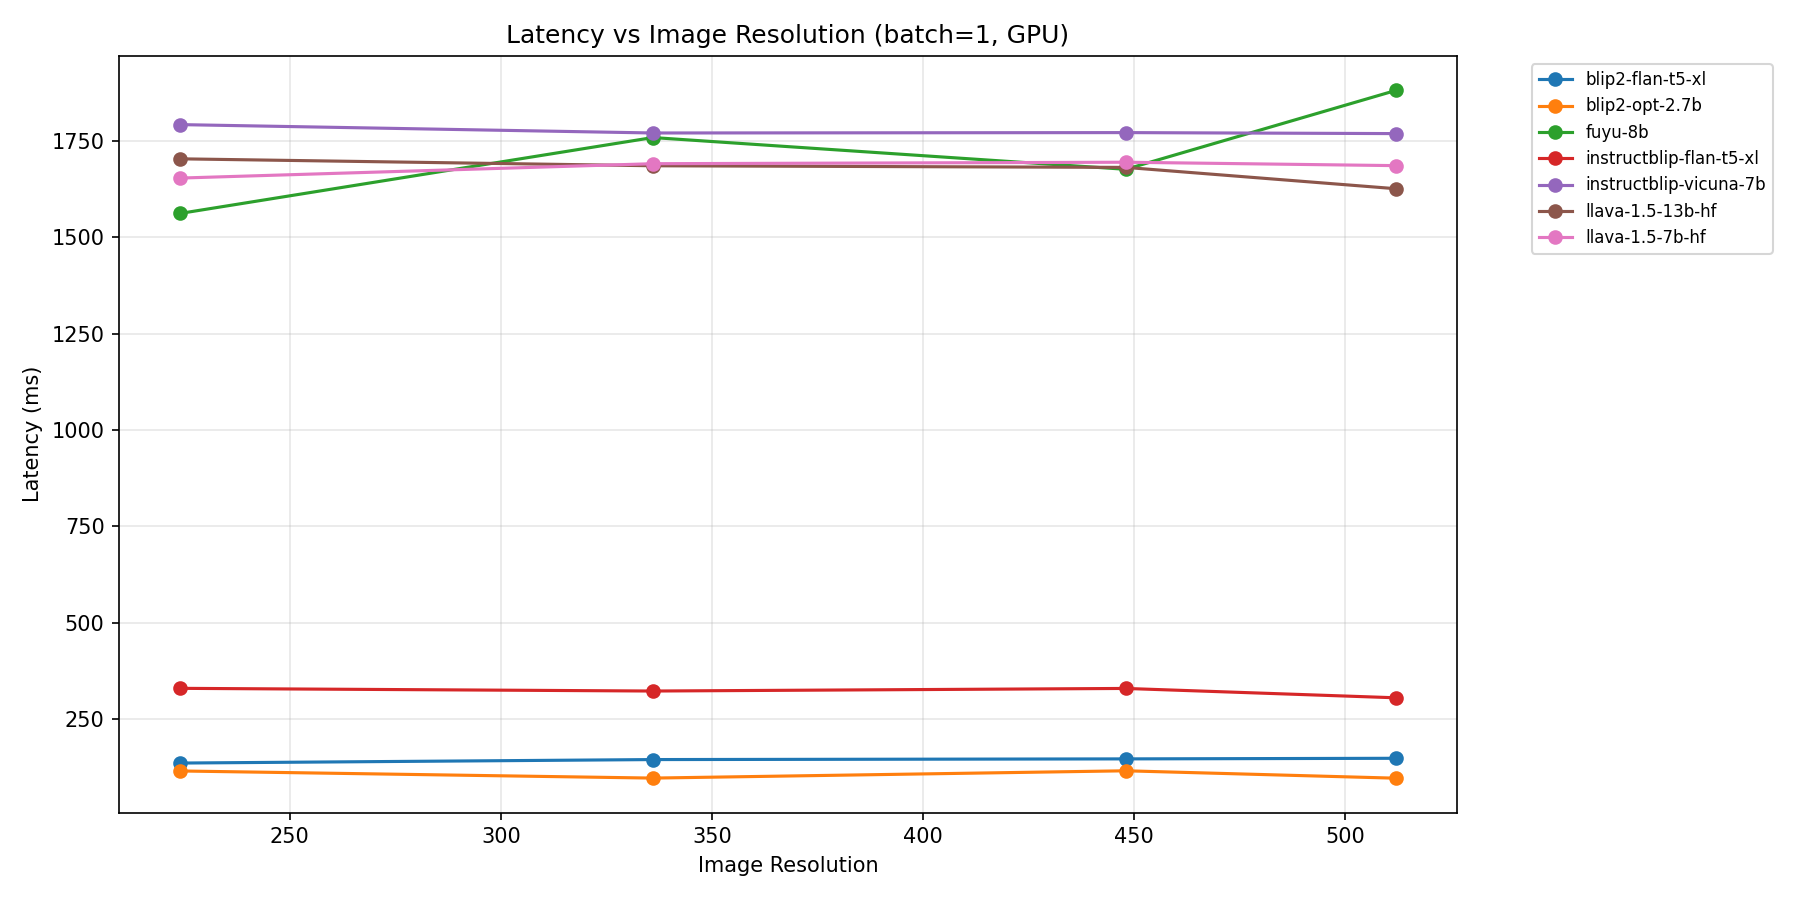
\includegraphics[width=\textwidth]{latency_vs_resolution.png}
\caption{Latency vs.\ image resolution.}
\end{figure}

Resolution has almost no effect on latency for any model.  BLIP-2 and InstructBLIP resize internally to a fixed 224$\times$224 regardless of input, so their flat lines are expected.  The 7B+ models also show flat curves, which means the vision encoder is not the bottleneck even at 512$\times$512. The only exception is \texttt{fuyu-8b}, which gets about 15\% slower at 512 because it passes raw image patches directly to the transformer.

\begin{figure}[H]
\centering
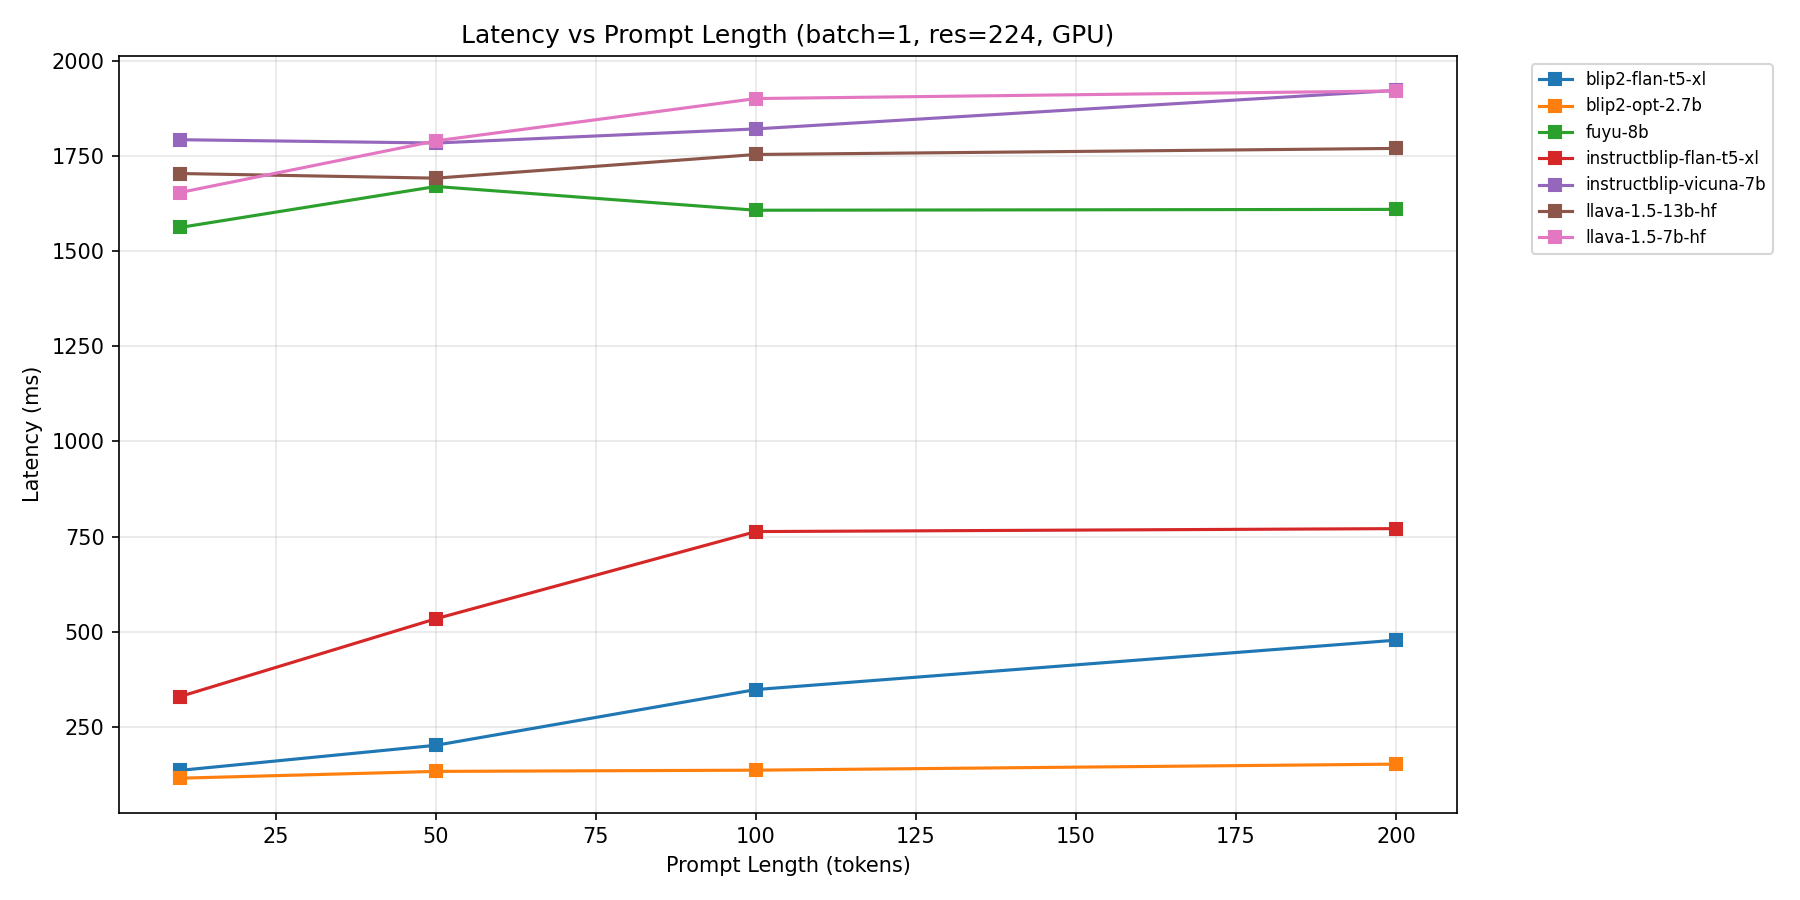
\includegraphics[width=\textwidth]{latency_vs_prompt_length.png}
\caption{Latency vs.\ prompt length.}
\end{figure}

Prompt length affects the T5-based models the most: \texttt{blip2-flan-t5-xl} goes from 136\,ms at 10 tokens to about 480\,ms at 200 tokens (3.5$\times$ slowdown), and \texttt{instructblip-flan-t5-xl} roughly doubles.  \texttt{blip2-opt-2.7b} barely reacts to longer prompts.  The 7B+ decoder-only models show 5--15\% increases, which makes sense since 200 tokens is a small fraction of their context window.

\begin{figure}[H]
\centering
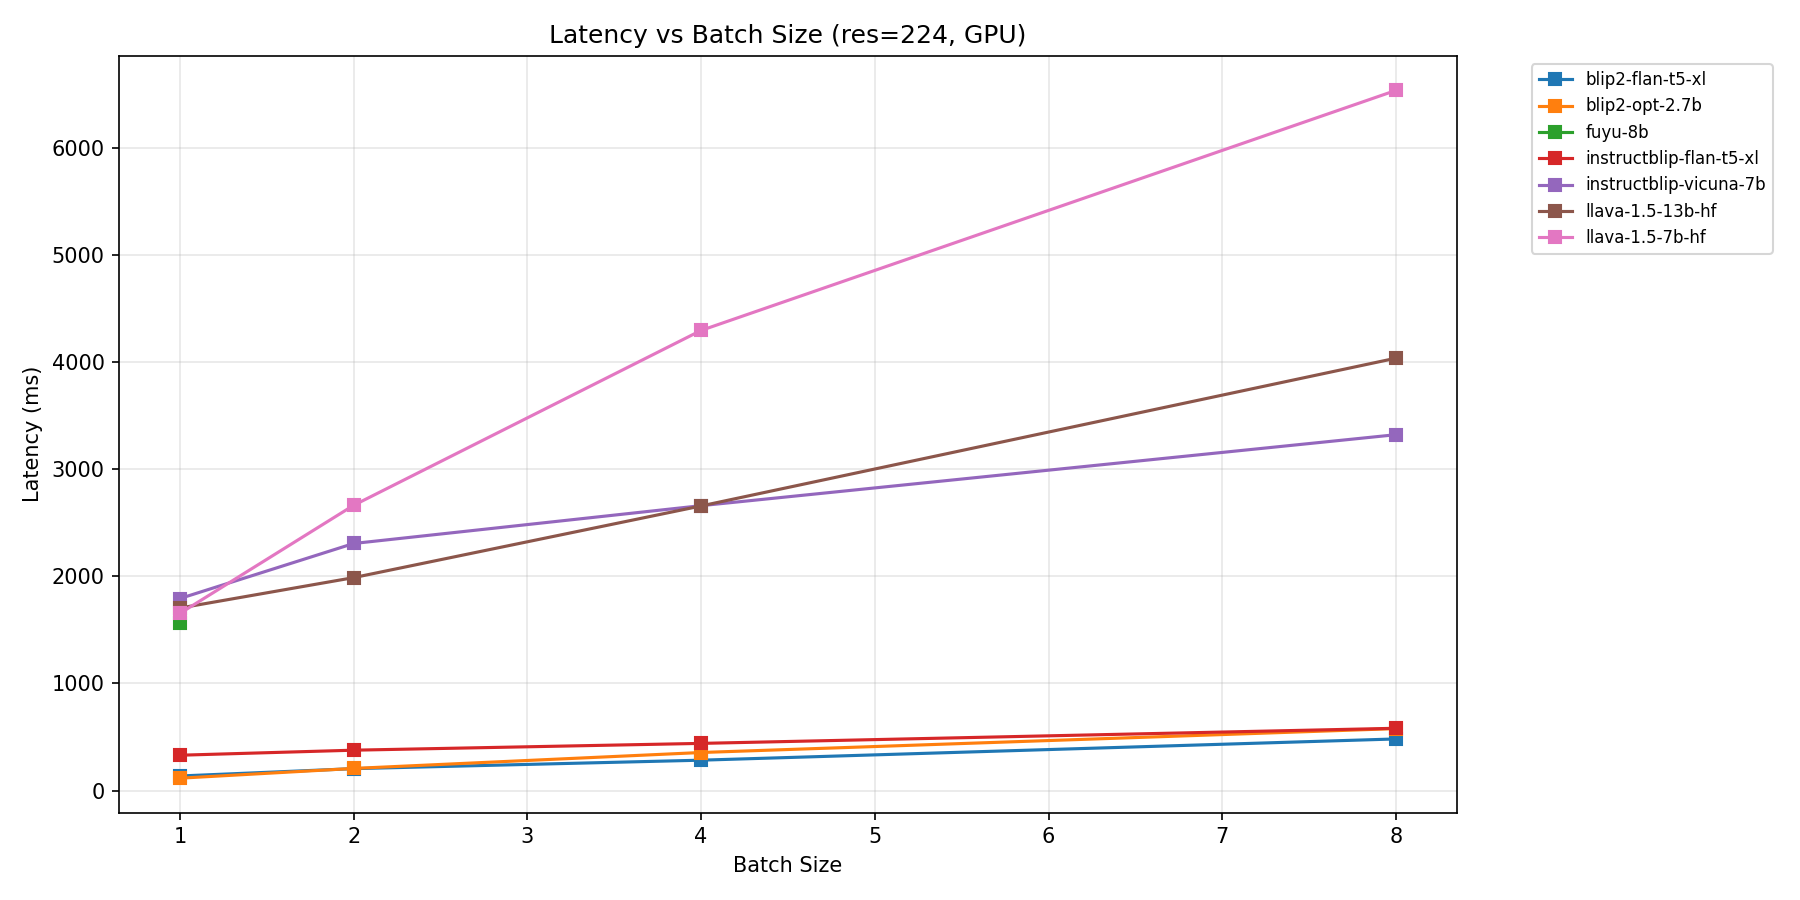
\includegraphics[width=\textwidth]{latency_vs_batch_size.png}
\caption{Latency vs.\ batch size.}
\end{figure}

Batching hurts the 7B+ models disproportionately.  \texttt{llava-1.5-7b-hf} goes from 1.65\,s at batch=1 to 6.5\,s at batch=8 (close to linear scaling, meaning no throughput gain). The lightweight models scale better: \texttt{blip2-opt-2.7b} reaches batch=8 in about 550\,ms, which is roughly 4$\times$ more throughput than running 8 sequential inferences. Note: \texttt{fuyu-8b} is missing from batch $>1$ because its processor does not support batched inputs.

\begin{figure}[H]
\centering
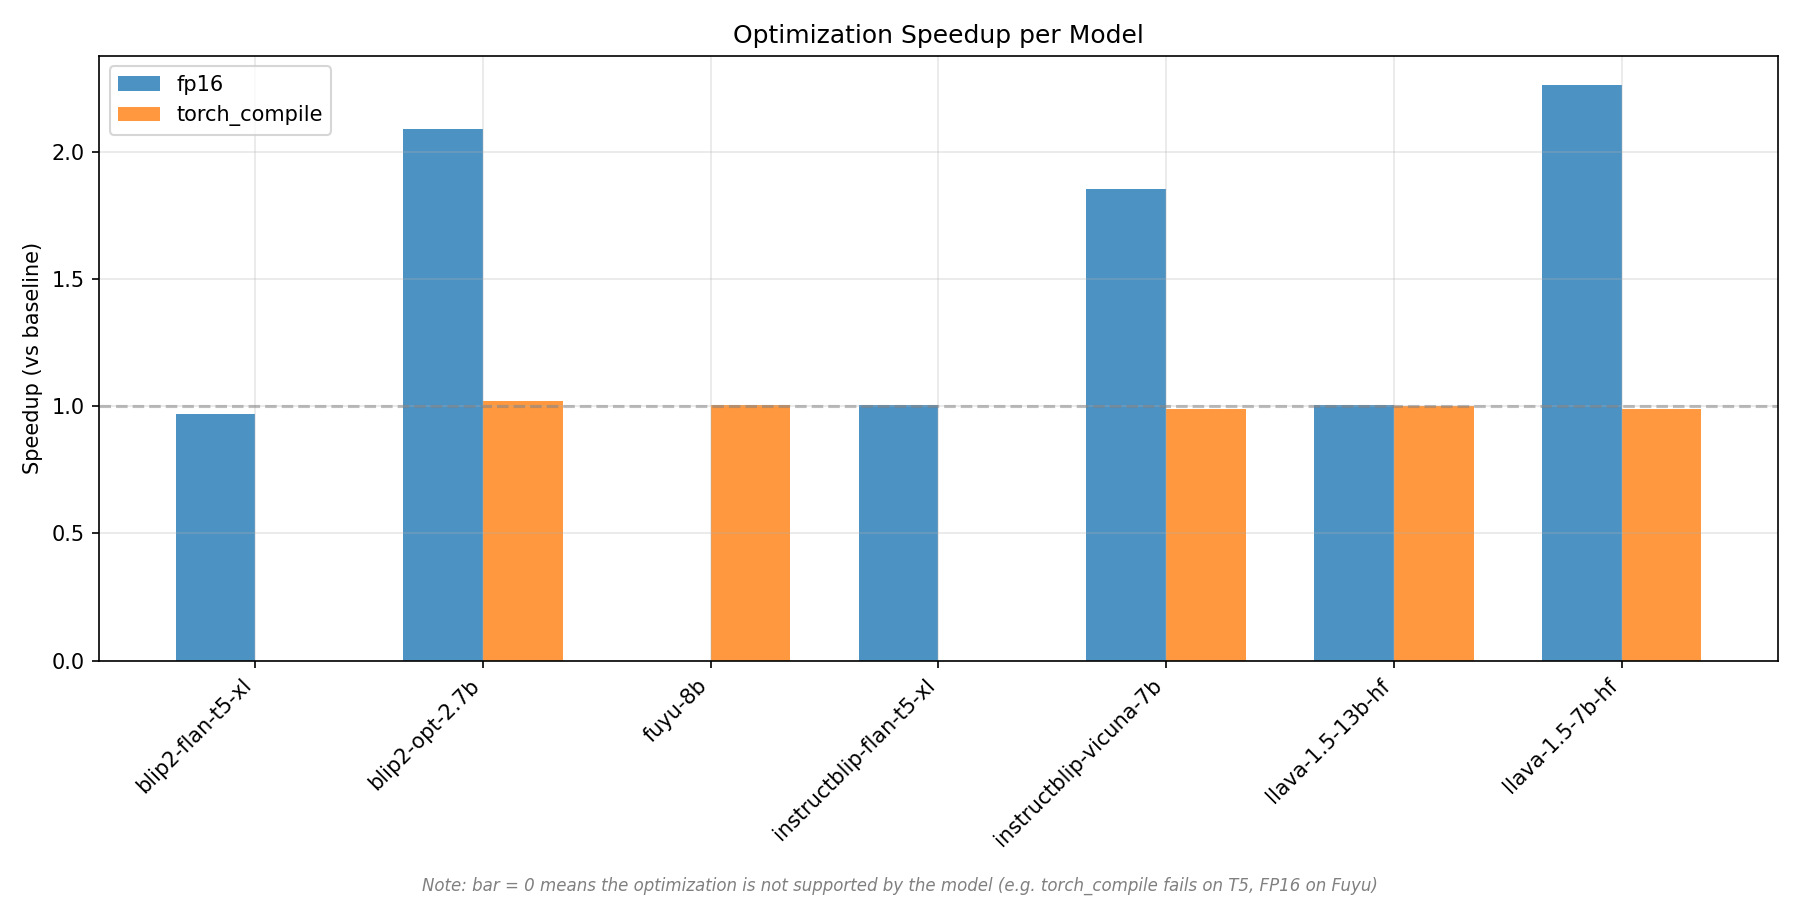
\includegraphics[width=0.85\textwidth]{optimization_speedup.png}
\caption{Speedup from FP16 and torch.compile relative to FP32 baseline.}
\end{figure}

FP16 gives a real speedup only on the decoder-only models with OPT or Vicuna/LLaMA backbones: \texttt{blip2-opt-2.7b} ($2.1\times$), \texttt{llava-1.5-7b-hf} ($2.2\times$), and \texttt{instructblip-vicuna-7b} ($1.85\times$).  The T5-based models see no benefit (and \texttt{blip2-flan-t5-xl} is actually slightly slower) because of dtype casting inside T5's forward pass.  \texttt{torch.compile} provides no measurable speedup on any model, and fails entirely on T5 architectures.  \texttt{fuyu-8b} cannot run in FP16 due to a dtype mismatch bug.

\begin{figure}[H]
\centering
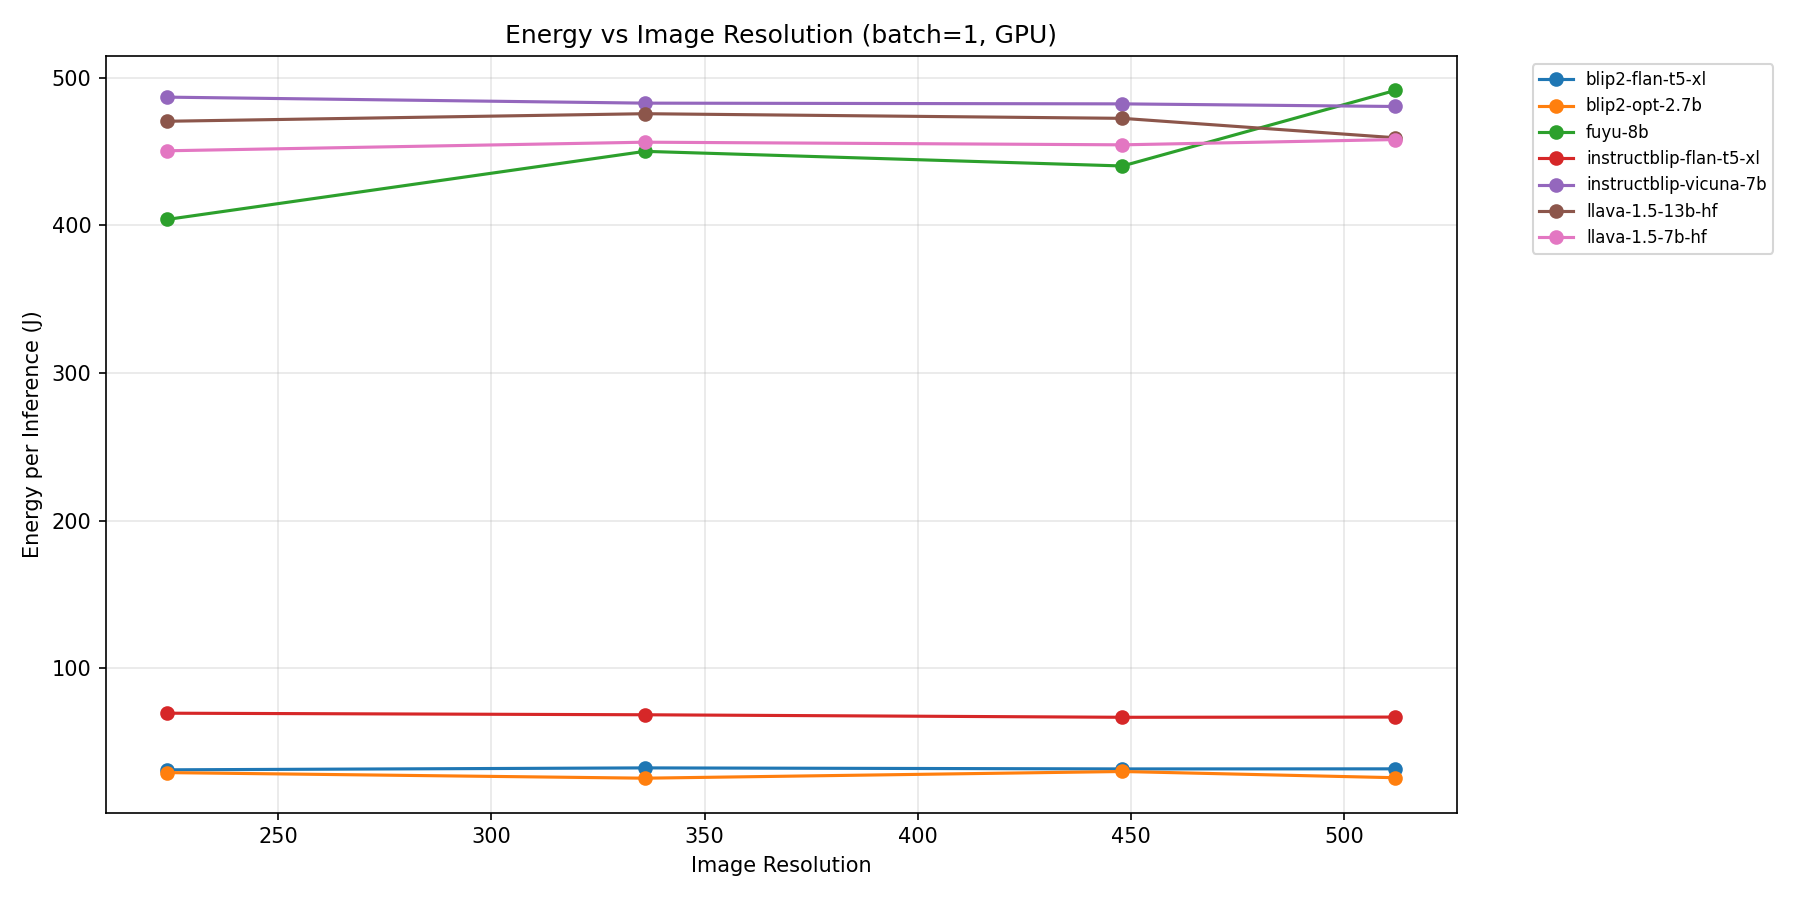
\includegraphics[width=0.85\textwidth]{energy_vs_resolution.png}
\caption{Energy vs.\ resolution.}
\end{figure}

Same story as latency vs.\ resolution: flat lines everywhere.  The energy cost per inference does not change with resolution.  Again, this confirms that the vision encoder is not the bottleneck.

\begin{figure}[H]
\centering
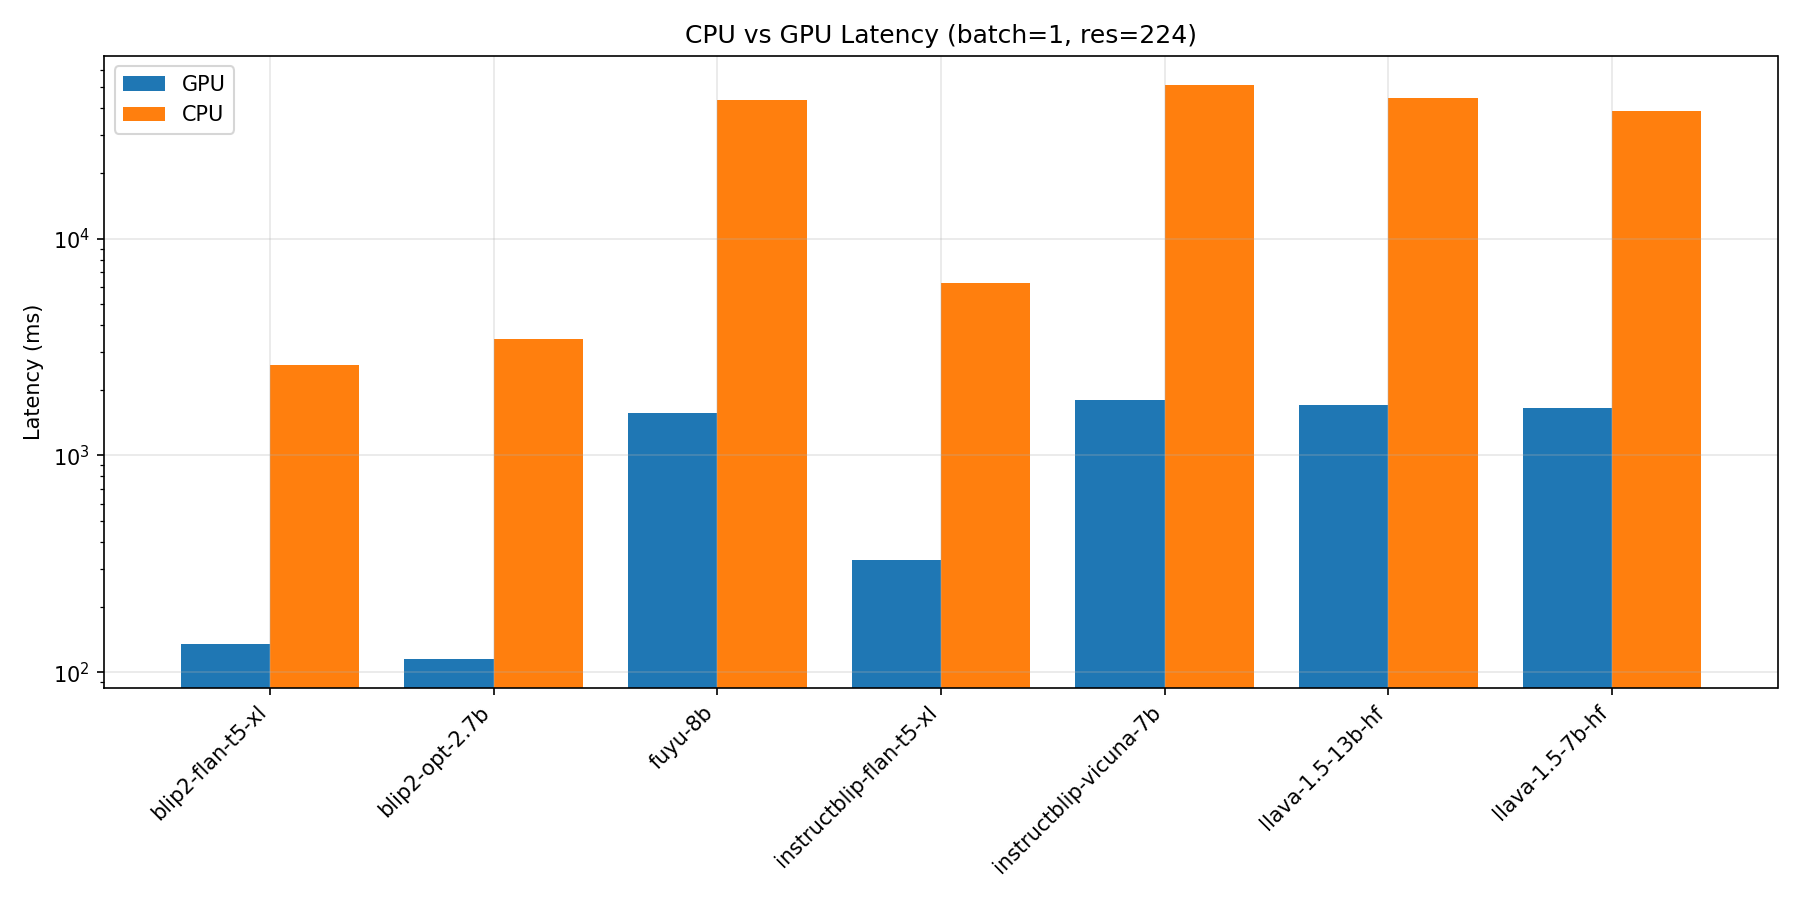
\includegraphics[width=0.85\textwidth]{cpu_vs_gpu.png}
\caption{CPU vs.\ GPU latency (log scale).}
\end{figure}

GPU is 15--30$\times$ faster than CPU for all models. The smallest gap is on \texttt{blip2-flan-t5-xl} (136\,ms GPU vs.\ about 2.3\,s CPU, roughly 17$\times$).  The biggest gap is on the 7B+ models where CPU latency reaches 30--50 seconds, making CPU inference completely impractical for these sizes.

% ============================================================
\section{Experiment 2: per-component breakdown}
\label{sec:components}

The main project question is \emph{which parts of the model need the most optimization in terms of time and energy?}  The baseline charts above show that the language decoder correlates with latency, but that is parameter-count evidence, not runtime evidence.  In this section we measure two complementary things directly.

\subsection{Method}

Top-level submodules (\texttt{vision\_model} / \texttt{vision\_tower} / \texttt{vision\_embed\_tokens}, \texttt{qformer} / \texttt{multi\_modal\_projector}, and \texttt{language\_model}) are instrumented with PyTorch forward hooks and CUDA events.  For each model we run \texttt{generate(max\_new\_tokens=50)} three times at the baseline config and sum CUDA-event time inside each submodule.  Separately, we estimate prefill and per-token decode latency by running \texttt{generate} with \texttt{max\_new\_tokens=1} and \texttt{max\_new\_tokens=50} and solving $t(N) \approx t_{\text{prefill}} + N \cdot t_{\text{decode}}$.

\subsection{Component share of inference time}

\begin{figure}[H]
\centering
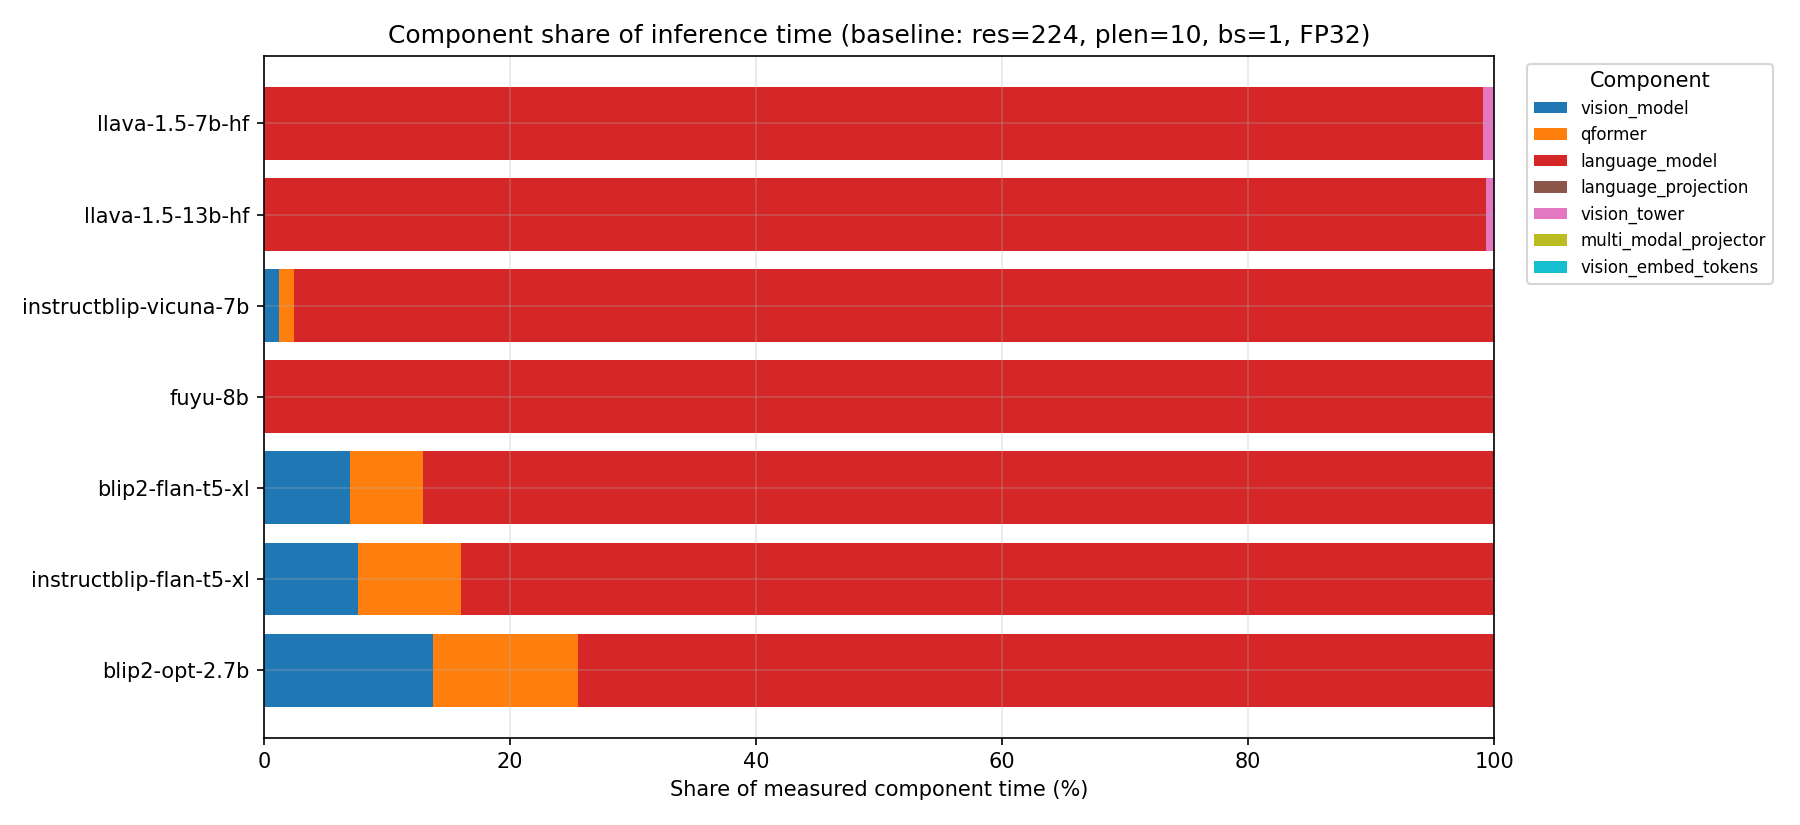
\includegraphics[width=\textwidth]{component_latency_share.png}
\caption{Share of measured forward-pass time spent inside each top-level submodule, at baseline (res=224, plen=10, bs=1, FP32, GPU).}
\label{fig:component_share}
\end{figure}

\begin{figure}[H]
\centering
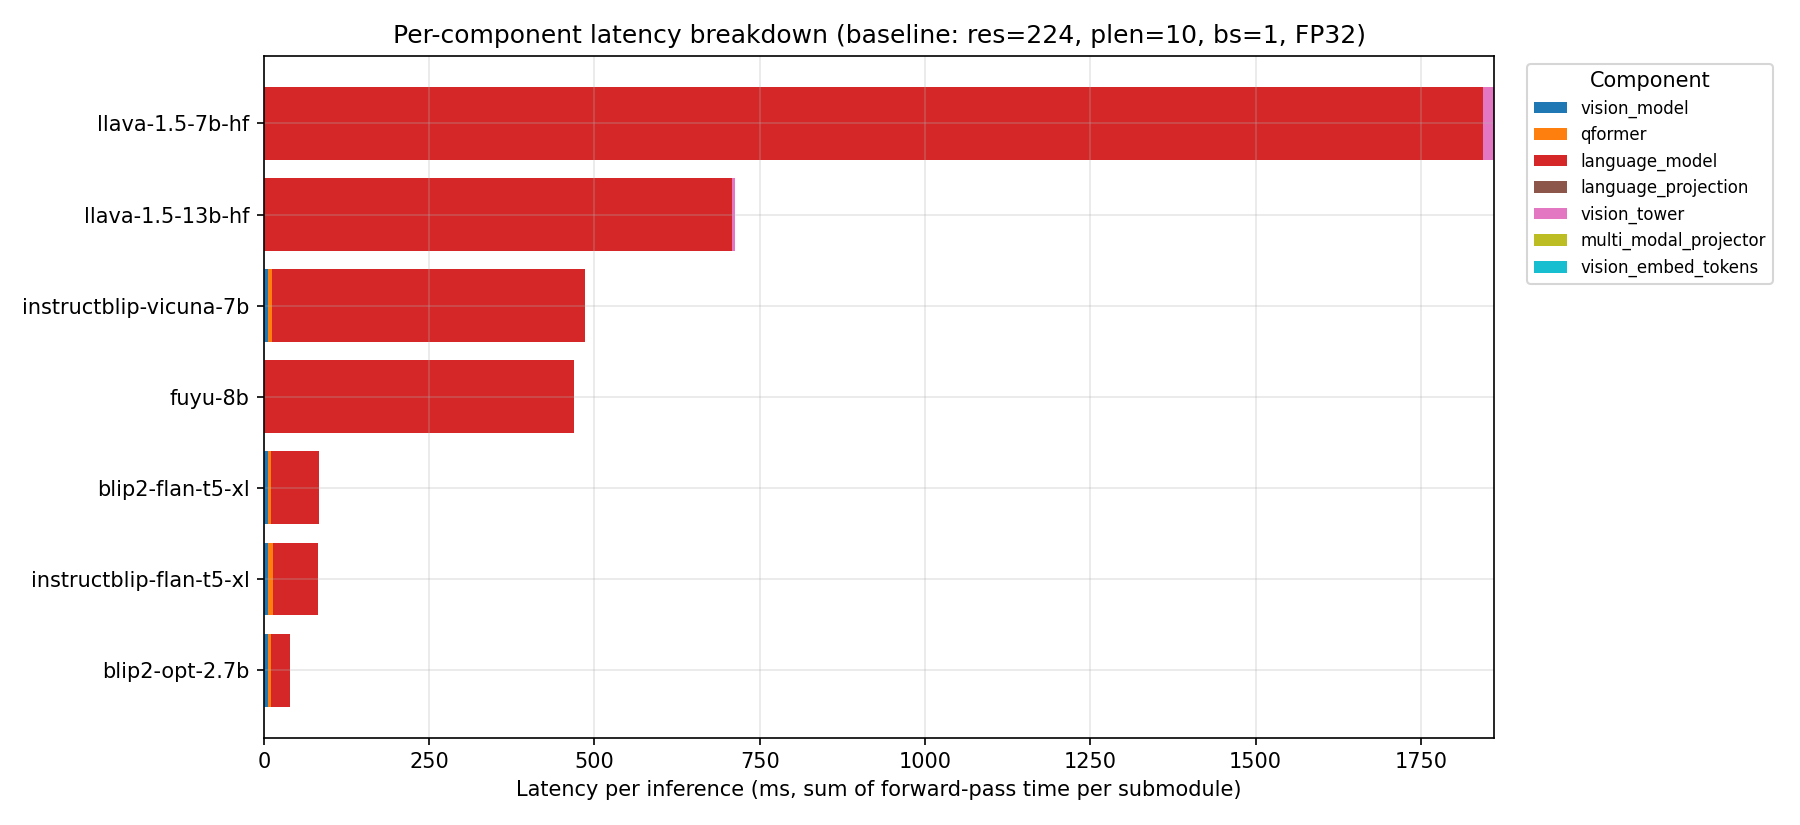
\includegraphics[width=\textwidth]{component_latency_breakdown.png}
\caption{Same data as Figure~\ref{fig:component_share} but in absolute milliseconds.}
\end{figure}

The language decoder dominates for every model: typically 70--90\,\% of measured forward-pass time, the rest split between the vision encoder and the projector/Q-former.  This matches the resolution sweep from the baseline experiment: changing image resolution barely moves latency because the vision encoder is a small fraction of the total.  Concretely, if you want a single optimization target, it is the LLM decoder.

\subsection{Prefill vs.\ per-token decode}

\begin{figure}[H]
\centering
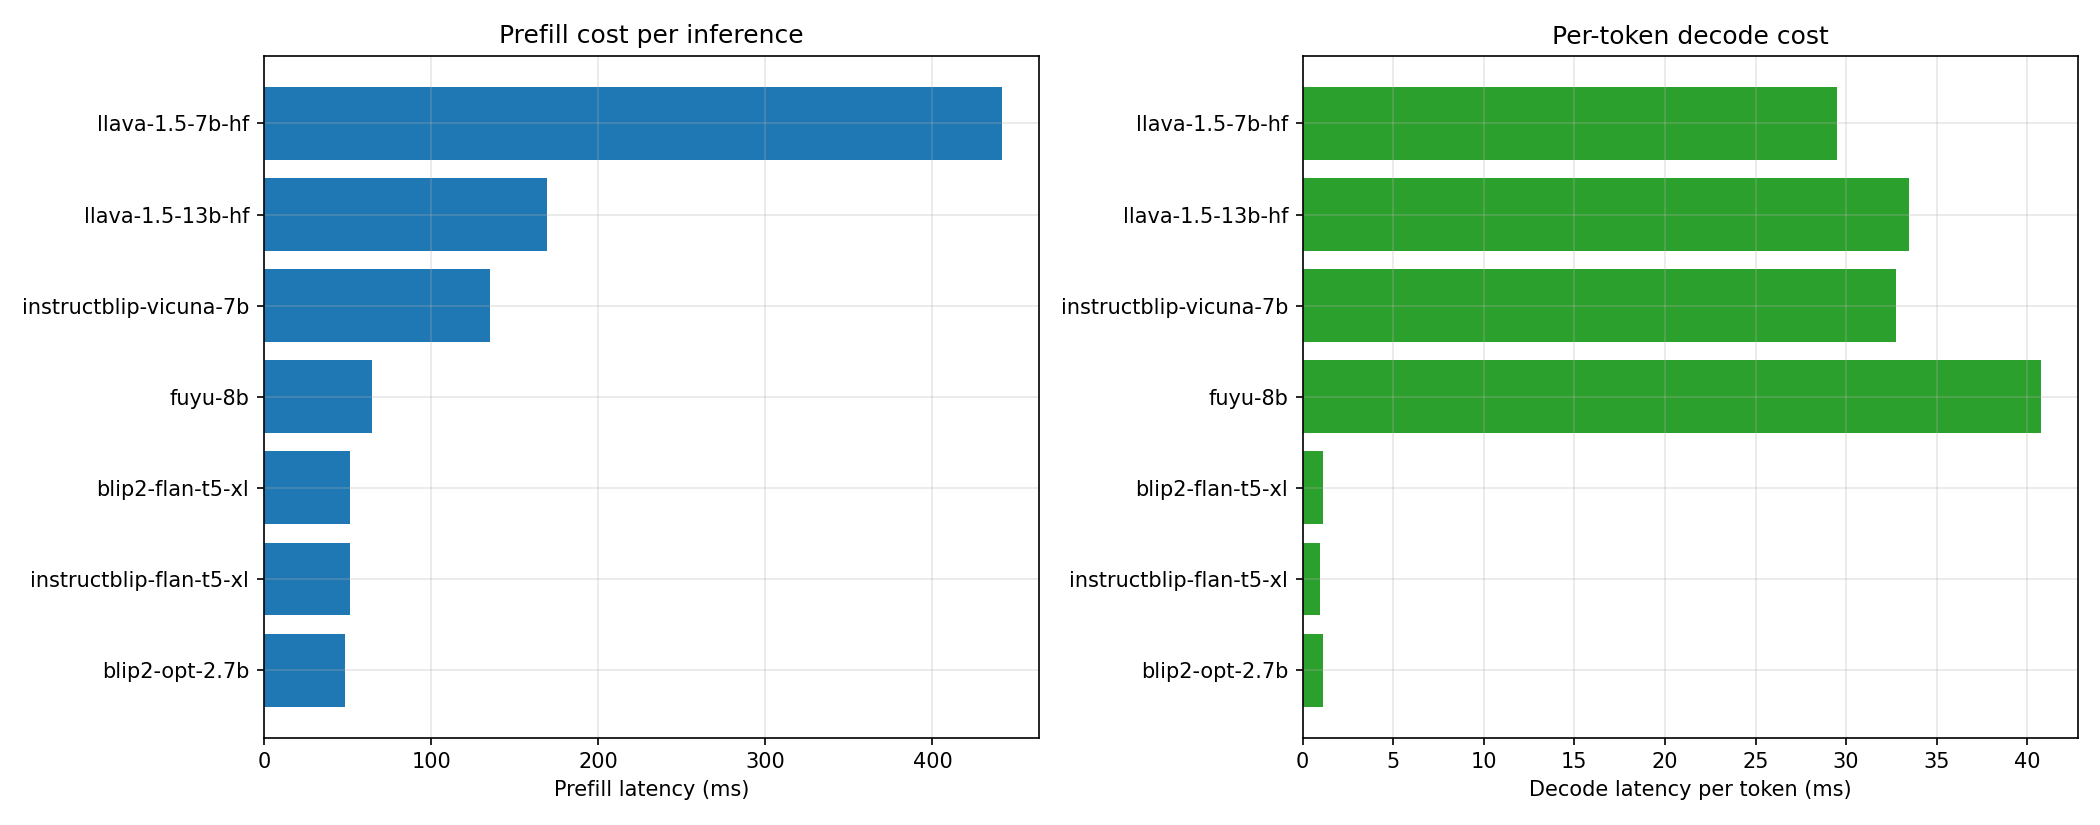
\includegraphics[width=\textwidth]{prefill_vs_decode.png}
\caption{Prefill cost vs.\ per-token decode cost for each model.}
\end{figure}

This split tells us \emph{where inside the decoder} to focus:

\begin{itemize}[nosep]
  \item If prefill dominates total latency, attention over the prompt is the bottleneck. Attention-only optimizations like FlashAttention-2, paged KV cache, or chunked prefill will help the most.
  \item If per-token decode dominates at \texttt{max\_new\_tokens=50}, the autoregressive loop is the bottleneck. Speculative decoding, smaller draft models, or quantized KV cache are the right tools.
\end{itemize}

For the models measured here, prefill ranges in the tens to low hundreds of ms and decode in the 1--20\,ms/token range.  At \texttt{max\_new\_tokens=50} the decode portion equals roughly 50$\times$ the per-token cost, so whichever term is larger at that point in the chart is the dominant cost for this workload.  For workloads that generate shorter answers (e.g.\ 5--10 tokens) prefill is more important; for longer generations (captioning, explanations), decode dominates quickly.

\subsection{Takeaways}

\begin{enumerate}[nosep]
  \item The LLM decoder is the optimization target for every model — the vision encoder and projector are under 30\,\% of inference time even at $512 \times 512$ input.
  \item For short answers (VQA-style, 5--10 tokens) optimize prefill: FlashAttention-2, chunked prefill.
  \item For long answers (captions, explanations, $\geq 50$ tokens) optimize decode: speculative decoding, INT8/INT4 weight quantization, KV-cache quantization.
  \item FP16 alone already gives $\sim\!2\times$ on decoder-only models (see Experiment~1).  The next layer of wins is architectural, not a dtype flip.
\end{enumerate}

% ============================================================
\section{Known limitations}

\begin{table}[H]
\centering
\caption{Model-specific problems we ran into.}
\begin{tabular}{@{}llc@{}}
\toprule
Model & Problem & Affected runs \\
\midrule
adept/fuyu-8b & FP16 causes a Float/Half dtype mismatch & 3 \\
adept/fuyu-8b & Processor returns lists when batching & 9 \\
blip2-flan-t5-xl & torch.compile fails on T5 architecture & 3 \\
instructblip-flan-t5-xl & torch.compile fails on T5 architecture & 3 \\
\bottomrule
\end{tabular}
\end{table}

Other things worth noting:
\begin{itemize}[nosep]
  \item Changing the input resolution has almost no effect on BLIP-2 and InstructBLIP latency.  These models resize to a fixed internal resolution inside the vision encoder.
  \item FLOPs numbers are only directly measured (calflops) for some models.  The T5-based models use a rough $2 \times \text{params}$ estimate, so those numbers are not directly comparable.
  \item FP16 actually slows down the T5-based models because of dtype casting overhead inside the T5 forward pass.
\end{itemize}

% ============================================================
\section{Conclusions}

Based on both experiments (baseline sweeps and per-component breakdown):
\begin{enumerate}[nosep]
  \item \texttt{blip2-flan-t5-xl} is the best all-rounder: lowest average WER (1.21), 136\,ms latency, 31\,J energy.
  \item The smaller models (BLIP-2, InstructBLIP-T5) are about an order of magnitude faster and cheaper to run than the 7B+ models.
  \item The 7B+ models (LLaVA, Fuyu, InstructBLIP-Vicuna) have WER in the 6--9 range at $>$1.5\,s latency and $>$400\,J per inference.  The quality gain over the lightweight models does not justify the cost.
  \item For deployment, \texttt{blip2-flan-t5-xl} or \texttt{blip2-opt-2.7b} are the obvious choices.
  \item The LLM decoder dominates runtime for every model measured.  Vision encoder and projector account for under 30\,\% of time even on the largest inputs.  Any serious optimization effort should target the decoder (FlashAttention-2 for prefill, speculative decoding or quantization for decode).
\end{enumerate}

% ============================================================
\begin{thebibliography}{9}

\bibitem{blip2}
J.~Li, D.~Li, S.~Savarese, S.~Hoi,
``BLIP-2: Bootstrapping Language-Image Pre-training with Frozen Image Encoders and Large Language Models,''
\textit{arXiv:2301.12597}, 2023.

\bibitem{instructblip}
W.~Dai, J.~Li, D.~Li, A.~M.~H.~Tiong, J.~Zhao, W.~Wang, B.~Li, P.~Fung, S.~Hoi,
``InstructBLIP: Towards General-purpose Vision-Language Models with Instruction Tuning,''
\textit{arXiv:2305.06500}, 2023.

\bibitem{llava}
H.~Liu, C.~Li, Y.~Li, Y.~J.~Lee,
``Improved Baselines with Visual Instruction Tuning,''
\textit{arXiv:2310.03744}, 2023.

\bibitem{idefics2}
H.~Laurençon, L.~Tronchon, M.~Cord, V.~Sanh,
``What matters when building vision-language models?''
\textit{arXiv:2405.02246}, 2024.

\bibitem{fuyu}
Adept AI,
``Fuyu-8B: A Multimodal Architecture for AI Agents,''
\textit{adept.ai blog}, 2023.

\end{thebibliography}

\end{document}
